\documentclass[12pt,a4paper]{article}

% --------------------------------------------------
% PACKAGES
% --------------------------------------------------
\usepackage[utf8]{inputenc}
\usepackage[T1]{fontenc}
\usepackage{lmodern}
\usepackage{geometry}
\usepackage{setspace}
\usepackage{graphicx}
\usepackage{booktabs}
\usepackage{array}
\usepackage{longtable}
\usepackage{xcolor}
\usepackage{listings}
\usepackage{amsmath}
\usepackage{amssymb}
\usepackage{hyperref}
\usepackage{enumitem}
\usepackage{fancyhdr}
\usepackage{tikz}
\usepackage{float}
\usepackage{titlesec}
\usepackage{tcolorbox}

\usetikzlibrary{arrows.meta, positioning, shapes.geometric, fit}

% --------------------------------------------------
% PAGE SETUP
% --------------------------------------------------
\geometry{
    top=25mm,
    bottom=25mm,
    left=25mm,
    right=25mm
}

\onehalfspacing

% --------------------------------------------------
% COLORS
% --------------------------------------------------
\definecolor{darkblue}{RGB}{25,55,100}
\definecolor{lightblue}{RGB}{235,242,250}
\definecolor{darkgray}{RGB}{60,60,60}
\definecolor{codegray}{RGB}{245,245,245}

% --------------------------------------------------
% HYPERLINKS
% --------------------------------------------------
\hypersetup{
    colorlinks=true,
    linkcolor=darkblue,
    urlcolor=darkblue,
    citecolor=darkblue,
    pdftitle={True Internet Bonding System},
    pdfauthor={Project Architecture Document}
}

% --------------------------------------------------
% HEADER / FOOTER
% --------------------------------------------------
\pagestyle{fancy}
\fancyhf{}
\fancyhead[L]{True Internet Bonding System}
\fancyhead[R]{Architecture Specification}
\fancyfoot[C]{\thepage}

% --------------------------------------------------
% CODE STYLE
% --------------------------------------------------
\lstset{
    backgroundcolor=\color{codegray},
    basicstyle=\ttfamily\small,
    breaklines=true,
    frame=single,
    columns=fullflexible
}

% --------------------------------------------------
% TITLE STYLE
% --------------------------------------------------
\titleformat{\section}
{\Large\bfseries\color{darkblue}}
{\thesection}
{1em}
{}

\titleformat{\subsection}
{\large\bfseries\color{darkgray}}
{\thesubsection}
{1em}
{}

% --------------------------------------------------
% DOCUMENT
% --------------------------------------------------
\begin{document}

% ==================================================
% TITLE PAGE
% ==================================================

\begin{titlepage}
    \centering

    \vspace*{2cm}

    {\Huge\bfseries True Internet Bonding System\par}

    \vspace{0.5cm}

    {\Large Multi-Path Internet Connection Bonding\par}

    \vspace{1.5cm}

    \begin{tcolorbox}[
        colback=lightblue,
        colframe=darkblue,
        width=0.9\textwidth
    ]
    \centering
    \textbf{Architecture Analysis and Technical Specification}
    \end{tcolorbox}

    \vspace{2cm}

    {\large
    Windows Client + Linux VPS\\
    Multi-Path Networking Architecture
    \par}

    \vfill

    {\large
    Project Architecture Document\\
    Version 1.0
    \par}

    \vspace{1cm}

    {\today}

\end{titlepage}

% ==================================================
% TABLE OF CONTENTS
% ==================================================

\tableofcontents
\newpage

% ==================================================
% 1. PROJECT OVERVIEW
% ==================================================

\section{Project Overview}

The objective of this project is to develop a true Internet Connection Bonding system capable of combining multiple independent Internet connections available on a Windows computer.

For example, a computer may simultaneously have:

\begin{itemize}
    \item Ethernet: 10 Mbps
    \item Wi-Fi: 2 Mbps
    \item USB Tethering: 3 Mbps
\end{itemize}

The theoretical aggregate bandwidth is:

\[
10 + 2 + 3 = 15\text{ Mbps}
\]

The purpose of the system is to allow these independent paths to participate in a single logical Internet connection.

The project is therefore not simply a network load balancer. It aims to implement actual multi-path Internet bonding in which traffic belonging to a logical connection can be distributed across multiple physical Internet paths and reconstructed at a remote bonding server.

\subsection{Important Technical Clarification}

The theoretical sum of all interfaces does not guarantee the same real-world throughput.

Actual throughput depends on:

\begin{itemize}
    \item Network latency
    \item Packet loss
    \item Jitter
    \item Protocol overhead
    \item Encryption overhead
    \item VPS bandwidth
    \item Server processing capacity
    \item Path asymmetry
    \item Congestion
\end{itemize}

Therefore, the system should aim to approach the aggregate capacity rather than guarantee an exact value.

% ==================================================
% 2. PROJECT GOAL
% ==================================================

\section{Project Goal}

The primary goal is to create a system with the following architecture:

\begin{center}
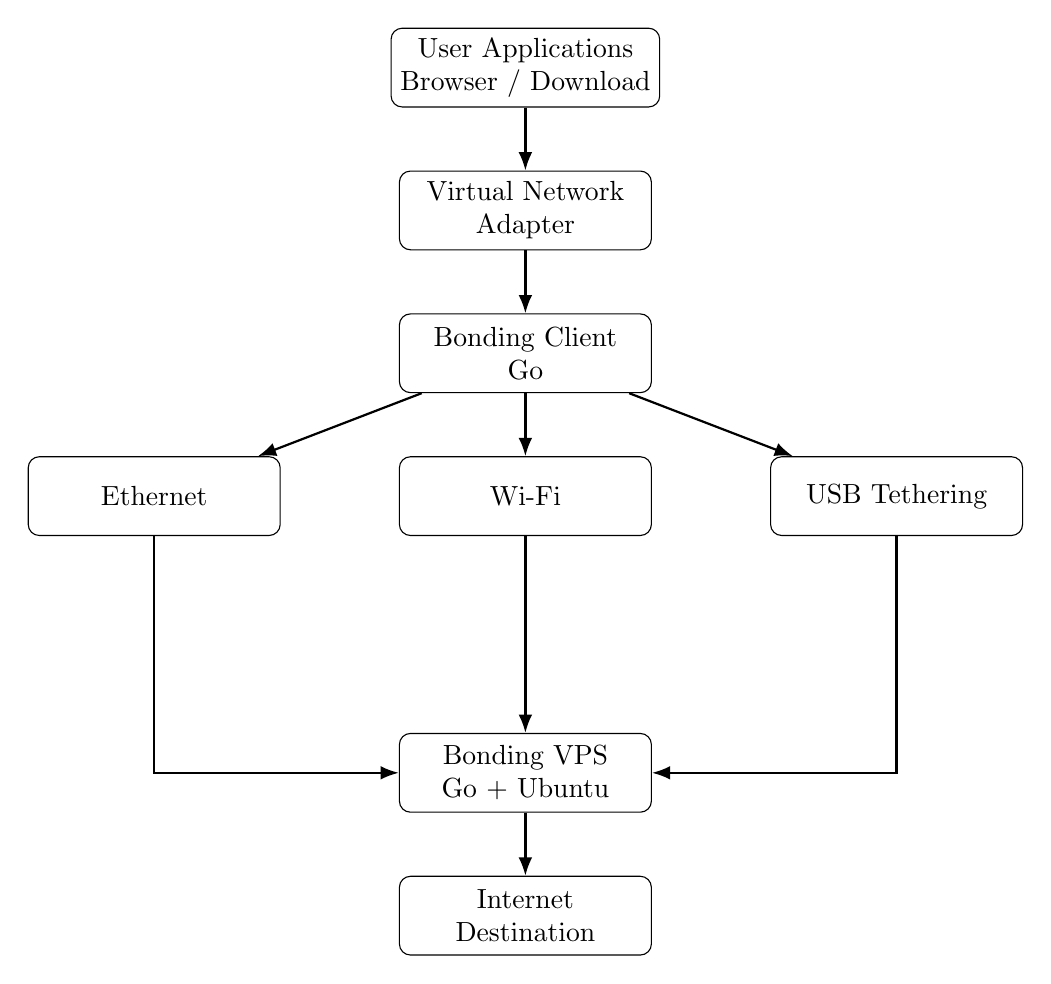
\begin{tikzpicture}[
    node distance=8mm and 15mm,
    box/.style={
        draw,
        rounded corners,
        align=center,
        minimum width=32mm,
        minimum height=10mm
    },
    arrow/.style={
        -{Latex},
        thick
    }
]

\node[box] (apps) {User Applications\\Browser / Download};

\node[box, below=of apps] (virtual) {Virtual Network\\Adapter};

\node[box, below=of virtual] (client) {Bonding Client\\Go};

\node[box, below left=of client] (eth) {Ethernet};
\node[box, below=of client] (wifi) {Wi-Fi};
\node[box, below right=of client] (usb) {USB Tethering};

\node[box, below=25mm of wifi] (vps) {Bonding VPS\\Go + Ubuntu};

\node[box, below=of vps] (internet) {Internet\\Destination};

\draw[arrow] (apps) -- (virtual);
\draw[arrow] (virtual) -- (client);

\draw[arrow] (client) -- (eth);
\draw[arrow] (client) -- (wifi);
\draw[arrow] (client) -- (usb);

\draw[arrow] (eth) |- (vps);
\draw[arrow] (wifi) -- (vps);
\draw[arrow] (usb) |- (vps);

\draw[arrow] (vps) -- (internet);

\end{tikzpicture}
\end{center}

% ==================================================
% 3. HIGH LEVEL ARCHITECTURE
% ==================================================

\section{High-Level Architecture}

The complete system consists of two major networking components:

\begin{enumerate}
    \item Windows Bonding Client
    \item Linux Bonding Server
\end{enumerate}

The Windows client receives traffic from applications through a virtual network interface.

The bonding engine then distributes packets across available physical Internet connections.

The remote VPS receives packets from all paths, reconstructs the logical traffic stream, and forwards the traffic to the Internet.

% ==================================================
% 4. CLIENT ARCHITECTURE
% ==================================================

\section{Windows Client Architecture}

The client runs on Windows 10/11 and contains the following major modules:

\begin{itemize}
    \item Virtual Network Adapter
    \item Network Adapter Manager
    \item Path Manager
    \item Packet Engine
    \item Packet Scheduler
    \item Reorder Buffer
    \item Loss Recovery
    \item Health Monitor
    \item Tunnel Manager
    \item Security Layer
    \item Session Manager
\end{itemize}

\subsection{Client Architecture Diagram}

\begin{center}
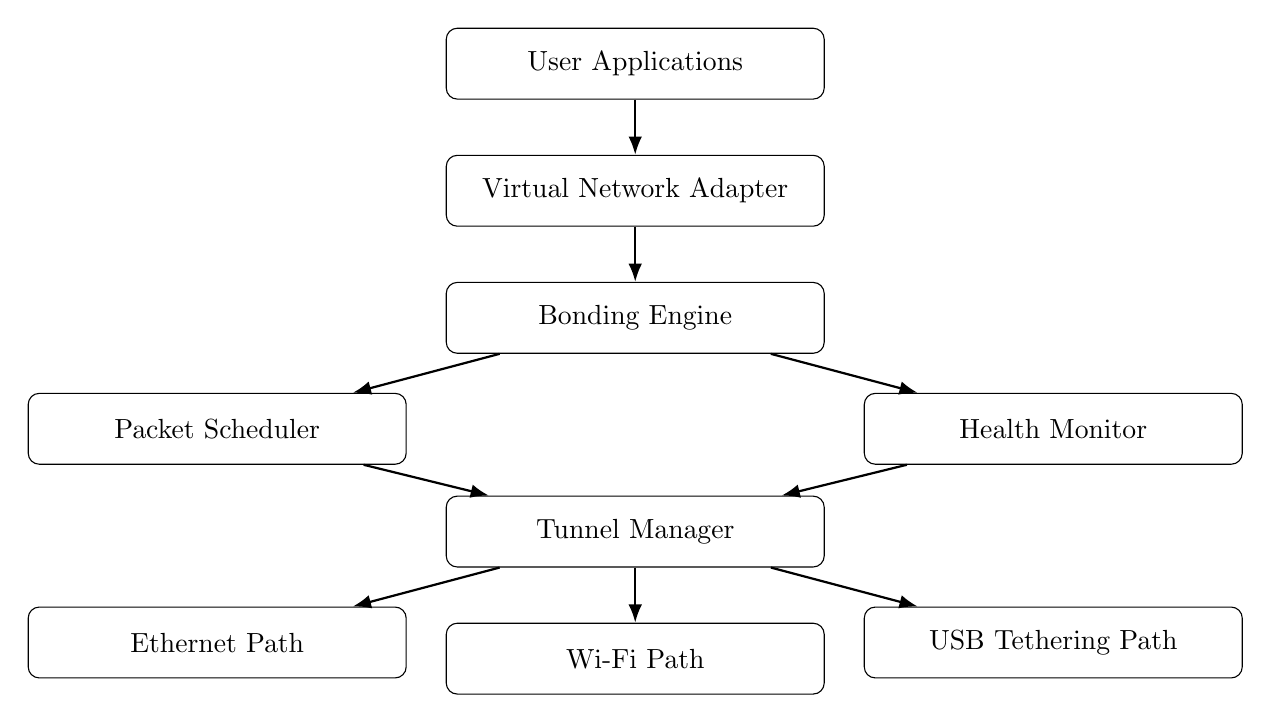
\begin{tikzpicture}[
    node distance=7mm,
    box/.style={
        draw,
        rounded corners,
        align=center,
        minimum width=48mm,
        minimum height=9mm
    },
    arrow/.style={
        -{Latex},
        thick
    }
]

\node[box] (app) {User Applications};

\node[box, below=of app] (adapter)
{Virtual Network Adapter};

\node[box, below=of adapter] (engine)
{Bonding Engine};

\node[box, below left=of engine] (scheduler)
{Packet Scheduler};

\node[box, below right=of engine] (monitor)
{Health Monitor};

\node[box, below=18mm of engine] (tunnel)
{Tunnel Manager};

\node[box, below left=of tunnel] (ethernet)
{Ethernet Path};

\node[box, below=of tunnel] (wifi)
{Wi-Fi Path};

\node[box, below right=of tunnel] (usb)
{USB Tethering Path};

\draw[arrow] (app) -- (adapter);
\draw[arrow] (adapter) -- (engine);

\draw[arrow] (engine) -- (scheduler);
\draw[arrow] (engine) -- (monitor);

\draw[arrow] (scheduler) -- (tunnel);
\draw[arrow] (monitor) -- (tunnel);

\draw[arrow] (tunnel) -- (ethernet);
\draw[arrow] (tunnel) -- (wifi);
\draw[arrow] (tunnel) -- (usb);

\end{tikzpicture}
\end{center}

% ==================================================
% 5. SERVER ARCHITECTURE
% ==================================================

\section{Bonding Server Architecture}

The remote server will run on Ubuntu Linux.

Its primary responsibilities are:

\begin{enumerate}
    \item Accept multiple tunnels from the client.
    \item Authenticate the client.
    \item Associate tunnels with a bonding session.
    \item Receive packets from multiple paths.
    \item Validate packets.
    \item Reorder packets.
    \item Handle missing packets.
    \item Reconstruct logical traffic.
    \item Forward traffic to the Internet.
    \item Receive response traffic.
    \item Distribute response traffic through available paths.
\end{enumerate}

\subsection{Server Diagram}

\begin{center}
\begin{tikzpicture}[
    node distance=8mm,
    box/.style={
        draw,
        rounded corners,
        align=center,
        minimum width=50mm,
        minimum height=10mm
    },
    arrow/.style={
        -{Latex},
        thick
    }
]

\node[box] (paths)
{Multiple Client Tunnels};

\node[box, below=of paths]
{Session Manager};

\node[box, below=of paths, xshift=-35mm]
{Tunnel Manager};

\node[box, below=of paths, xshift=35mm]
{Packet Validation};

\node[box, below=22mm of paths]
{Reassembly / Reordering};

\node[box, below=of reassembly]
{Routing + NAT};

\node[box, below=of routing]
{Internet};

\end{tikzpicture}
\end{center}

% ==================================================
% 6. TECHNOLOGY STACK
% ==================================================

\section{Technology Stack}

\begin{longtable}{p{0.28\textwidth} p{0.62\textwidth}}
\toprule
\textbf{Component} & \textbf{Technology} \\
\midrule
Client Core & Go \\
Server Core & Go \\
Client OS & Windows 10/11 \\
Server OS & Ubuntu Linux \\
Virtual Networking & Wintun / Windows networking APIs \\
Packet Interception & WinDivert or Windows Filtering Platform, if required \\
Initial Transport & UDP \\
Alternative Transport & QUIC \\
Encryption & TLS 1.3 or Noise-based protocol \\
Server Routing & Linux routing + nftables/iptables \\
NAT & Linux NAT \\
Dashboard & React + TypeScript + Tailwind CSS \\
Real-Time Communication & WebSocket \\
Testing & iperf3, Wireshark, ping, curl, tracert \\
Version Control & Git + GitHub \\
Development Assistant & Antigravity \\
\bottomrule
\end{longtable}

\subsection{Technology Selection Principle}

The project should avoid unnecessary technologies.

A database, message broker, Kubernetes cluster, or microservice architecture is not required for the initial bonding engine.

The core system should remain lightweight and networking-focused.

% ==================================================
% 7. MULTI-PATH MODEL
% ==================================================

\section{Multi-Path Networking Model}

Every physical Internet connection represents a separate network path.

For example:

\begin{itemize}
    \item Path 1: Ethernet
    \item Path 2: Wi-Fi
    \item Path 3: USB Tethering
\end{itemize}

Each path may have a different:

\begin{itemize}
    \item Public IP
    \item Latency
    \item Bandwidth
    \item Packet loss
    \item MTU
    \item Jitter
\end{itemize}

The bonding engine must treat each path independently.

% ==================================================
% 8. TUNNELS
% ==================================================

\section{Multi-Path Tunnels}

The client should maintain independent tunnels over the available paths.

Example:

\begin{verbatim}
Tunnel 1 -> Ethernet -> VPS
Tunnel 2 -> Wi-Fi -> VPS
Tunnel 3 -> USB -> VPS
\end{verbatim}

The bonding session associates all of these tunnels with one logical session.

% ==================================================
% 9. PACKET FORMAT
% ==================================================

\section{Bonding Packet Format}

A custom packet format is required to identify and manage traffic transmitted through different paths.

A possible header is:

\begin{center}
\begin{tabular}{|c|c|c|c|c|}
\hline
Version & Session ID & Path ID & Sequence No. & Payload \\
\hline
\end{tabular}
\end{center}

Additional fields may include:

\begin{itemize}
    \item Packet Type
    \item Timestamp
    \item Payload Length
    \item Flags
    \item Authentication Tag
\end{itemize}

The final packet format must consider:

\begin{itemize}
    \item MTU
    \item Fragmentation
    \item Encryption overhead
    \item Replay protection
    \item Integrity verification
\end{itemize}

% ==================================================
% 10. PACKET ORDERING
% ==================================================

\section{Packet Ordering and Reassembly}

Different Internet paths have different latency.

Therefore, packets can arrive out of order.

For example:

\begin{verbatim}
Sent:
100 101 102 103 104

Received:
100 102 103 101 104
\end{verbatim}

The receiver requires a reorder buffer.

\begin{center}
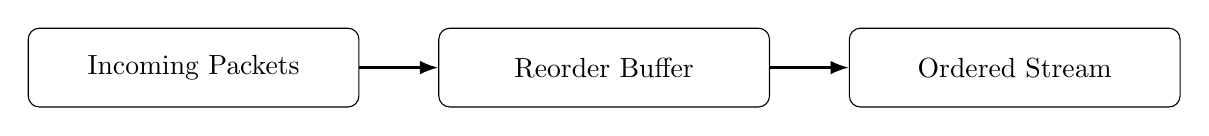
\begin{tikzpicture}[
    node distance=10mm,
    box/.style={
        draw,
        rounded corners,
        align=center,
        minimum width=42mm,
        minimum height=10mm
    },
    arrow/.style={
        -{Latex},
        thick
    }
]

\node[box] (incoming) {Incoming Packets};

\node[box, right=of incoming] (buffer)
{Reorder Buffer};

\node[box, right=of buffer] (ordered)
{Ordered Stream};

\draw[arrow] (incoming) -- (buffer);
\draw[arrow] (buffer) -- (ordered);

\end{tikzpicture}
\end{center}

The reorder buffer must support:

\begin{itemize}
    \item Sequence tracking
    \item Duplicate detection
    \item Missing packet detection
    \item Timeout handling
    \item Ordered delivery
\end{itemize}

% ==================================================
% 11. PACKET LOSS
% ==================================================

\section{Packet Loss and Recovery}

Internet paths can experience packet loss.

Example:

\begin{verbatim}
100
101
102
103
104
106
\end{verbatim}

Packet 105 is missing.

The receiver should detect the missing sequence number.

Possible recovery mechanisms include:

\begin{itemize}
    \item Retransmission request
    \item Selective retransmission
    \item Alternate path recovery
    \item Timeout-based recovery
\end{itemize}

The final strategy should be optimized for heterogeneous network paths.

% ==================================================
% 12. SCHEDULER
% ==================================================

\section{Traffic Scheduler}

The scheduler is responsible for deciding which path should carry each packet.

For example:

\[
Ethernet = 10 Mbps
\]

\[
WiFi = 2 Mbps
\]

\[
USB = 3 Mbps
\]

Total theoretical capacity:

\[
15 Mbps
\]

A simple weighted distribution could initially be:

\[
Ethernet \approx 66.7\%
\]

\[
WiFi \approx 13.3\%
\]

\[
USB \approx 20\%
\]

However, the final scheduler should use real-time network conditions.

\subsection{Scheduler Inputs}

\begin{itemize}
    \item Measured bandwidth
    \item RTT
    \item Packet loss
    \item Jitter
    \item Congestion
    \item Queue depth
    \item Path availability
\end{itemize}

\subsection{Candidate Algorithms}

The following algorithms should be evaluated:

\begin{enumerate}
    \item Weighted Round Robin
    \item Weighted Fair Queuing
    \item Least-Latency Scheduling
    \item Adaptive Weighted Scheduling
    \item Congestion-Aware Scheduling
\end{enumerate}

For the MVP, a simple adaptive weighted scheduler is recommended.

% ==================================================
% 13. BANDWIDTH MONITORING
% ==================================================

\section{Bandwidth and Path Monitoring}

The system must independently monitor every path.

Metrics include:

\begin{itemize}
    \item Throughput
    \item Latency
    \item RTT
    \item Packet loss
    \item Jitter
    \item Interface status
    \item Gateway availability
\end{itemize}

Windows-reported link speed should not be treated as actual Internet bandwidth.

Actual throughput must be measured through controlled traffic.

% ==================================================
% 14. WINDOWS VIRTUAL NETWORKING
% ==================================================

\section{Windows Virtual Networking}

The most important Windows component is the virtual networking layer.

The desired packet flow is:

\begin{verbatim}
Application
    |
    v
Virtual Network Adapter
    |
    v
Bonding Engine
    |
    +---- Ethernet
    |
    +---- Wi-Fi
    |
    +---- USB
    |
    v
Bonding VPS
    |
    v
Internet
\end{verbatim}

Potential technologies include:

\begin{itemize}
    \item Wintun
    \item WinDivert
    \item Windows Filtering Platform
    \item Windows routing APIs
\end{itemize}

The final architecture must determine which mechanism is actually required.

The system should avoid unnecessary packet interception layers.

% ==================================================
% 15. SERVER ROUTING
% ==================================================

\section{VPS Routing and NAT}

The VPS acts as the Internet-facing aggregation point.

Traffic flow:

\begin{verbatim}
Windows Client
      |
      v
Bonding Tunnels
      |
      v
VPS
      |
      v
NAT / Routing
      |
      v
Internet
\end{verbatim}

The VPS will require:

\begin{itemize}
    \item IP forwarding
    \item NAT
    \item Firewall rules
    \item Routing configuration
\end{itemize}

The VPS bandwidth must be greater than the expected aggregate client bandwidth.

% ==================================================
% 16. RETURN TRAFFIC
% ==================================================

\section{Return Traffic}

Download traffic is equally important.

The reverse path should be:

\begin{verbatim}
Internet
   |
   v
Bonding VPS
   |
   +---- Tunnel 1
   +---- Tunnel 2
   +---- Tunnel 3
   |
   v
Bonding Client
   |
   v
Virtual Network Adapter
   |
   v
Application
\end{verbatim}

The server therefore needs a strategy for distributing response traffic across available paths.

% ==================================================
% 17. SESSION MANAGEMENT
% ==================================================

\section{Session Management}

A bonding session should contain:

\begin{itemize}
    \item Session ID
    \item Client identity
    \item Authentication state
    \item Active tunnels
    \item Path status
    \item Keepalive state
    \item Session statistics
\end{itemize}

The system must support:

\begin{itemize}
    \item Reconnection
    \item Tunnel failure
    \item Client restart
    \item Server restart
    \item Path rejoining
\end{itemize}

% ==================================================
% 18. KEEPALIVE
% ==================================================

\section{Keepalive and Health Monitoring}

Each active path should have a health mechanism.

Example:

\begin{verbatim}
Client -> PING -> VPS
Client <- PONG <- VPS
\end{verbatim}

The system measures:

\begin{itemize}
    \item RTT
    \item Packet loss
    \item Availability
\end{itemize}

A failed path should automatically be removed from scheduling.

When the path becomes available again, it should be able to rejoin the bonding session.

% ==================================================
% 19. SECURITY
% ==================================================

\section{Security Architecture}

The system must protect against:

\begin{itemize}
    \item Unauthorized clients
    \item Packet injection
    \item Replay attacks
    \item Session hijacking
    \item Man-in-the-middle attacks
    \item Fake servers
    \item Denial-of-service attacks
\end{itemize}

Security mechanisms should include:

\begin{itemize}
    \item Strong client authentication
    \item Encryption
    \item Packet integrity
    \item Replay protection
    \item Secure key management
\end{itemize}

Secrets must never be hard-coded into source code.

% ==================================================
% 20. FAILURE HANDLING
% ==================================================

\section{Failure Handling}

\subsection{All Paths Healthy}

Example:

\begin{verbatim}
Ethernet = 10 Mbps
Wi-Fi    = 2 Mbps
USB      = 3 Mbps
\end{verbatim}

All paths participate in bonding.

\subsection{Wi-Fi Disconnects}

The system should automatically continue through Ethernet and USB.

\subsection{USB Becomes Unstable}

The scheduler should reduce or stop traffic through the USB path.

\subsection{Ethernet Disconnects}

The system should continue through remaining paths.

\subsection{High Latency}

A path with extreme latency should receive less traffic.

% ==================================================
% 21. MVP
% ==================================================

\section{Minimum Viable Product}

The first MVP should NOT attempt to implement every feature.

The MVP should contain:

\begin{enumerate}
    \item Windows client
    \item Linux VPS
    \item Two Internet paths
    \item UDP tunnels
    \item Session management
    \item Packet sequence numbers
    \item Packet scheduling
    \item Packet reordering
    \item Basic loss recovery
    \item Virtual network interface
    \item Single logical Internet connection
\end{enumerate}

The first physical test should use:

\begin{itemize}
    \item Ethernet
    \item Wi-Fi
\end{itemize}

USB tethering should be added only after the two-path implementation works reliably.

% ==================================================
% 22. DEVELOPMENT PHASES
% ==================================================

\section{Development Roadmap}

\subsection{Phase 1 -- Network Discovery}

Implement:

\begin{itemize}
    \item Network interface detection
    \item IP address detection
    \item Gateway detection
    \item Interface status
\end{itemize}

\subsection{Phase 2 -- Path Monitoring}

Implement:

\begin{itemize}
    \item RTT measurement
    \item Packet loss measurement
    \item Throughput measurement
    \item Health monitoring
\end{itemize}

\subsection{Phase 3 -- Client to VPS Tunnel}

Implement:

\begin{itemize}
    \item UDP tunnel
    \item Authentication
    \item Keepalive
    \item Session establishment
\end{itemize}

\subsection{Phase 4 -- Multiple Tunnels}

Implement:

\begin{itemize}
    \item Ethernet tunnel
    \item Wi-Fi tunnel
    \item Independent path identification
\end{itemize}

\subsection{Phase 5 -- Bonding Protocol}

Implement:

\begin{itemize}
    \item Packet format
    \item Sequence numbers
    \item Path IDs
    \item Session IDs
\end{itemize}

\subsection{Phase 6 -- Scheduler}

Implement:

\begin{itemize}
    \item Weighted scheduling
    \item Adaptive path selection
    \item Path health integration
\end{itemize}

\subsection{Phase 7 -- Reordering and Recovery}

Implement:

\begin{itemize}
    \item Reorder buffer
    \item Missing packet detection
    \item Selective retransmission
\end{itemize}

\subsection{Phase 8 -- Virtual Network Interface}

Integrate:

\begin{itemize}
    \item Wintun or selected Windows networking mechanism
    \item Application traffic interception
    \item Packet forwarding
\end{itemize}

\subsection{Phase 9 -- True Two-Path Bonding}

Test:

\begin{verbatim}
Ethernet + Wi-Fi
        |
        v
Single logical connection
        |
        v
VPS
        |
        v
Internet
\end{verbatim}

\subsection{Phase 10 -- USB Tethering}

Add:

\begin{verbatim}
Ethernet + Wi-Fi + USB
\end{verbatim}

\subsection{Phase 11 -- Dashboard}

Build:

\begin{itemize}
    \item React interface
    \item Real-time metrics
    \item Connection status
    \item Combined bandwidth
    \item Latency
    \item Packet loss
\end{itemize}

\subsection{Phase 12 -- Production Hardening}

Implement:

\begin{itemize}
    \item Windows service
    \item Auto-start
    \item Secure configuration
    \item Logging
    \item Diagnostics
    \item Performance optimization
\end{itemize}

% ==================================================
% 23. REPOSITORY STRUCTURE
% ==================================================

\section{Repository Structure}

The recommended repository structure is:

\begin{verbatim}
internet-bonding/
|
+-- client/
|   +-- cmd/
|   |   +-- bonding-client/
|   |       +-- main.go
|   |
|   +-- internal/
|   |   +-- adapter/
|   |   +-- packet/
|   |   +-- scheduler/
|   |   +-- tunnel/
|   |   +-- reorder/
|   |   +-- recovery/
|   |   +-- monitor/
|   |   +-- security/
|   |   +-- session/
|   |   +-- platform/
|   |
|   +-- config/
|   +-- tests/
|
+-- server/
|   +-- cmd/
|   |   +-- bonding-server/
|   |       +-- main.go
|   |
|   +-- internal/
|       +-- session/
|       +-- tunnel/
|       +-- packet/
|       +-- reassembly/
|       +-- recovery/
|       +-- routing/
|       +-- nat/
|       +-- security/
|
+-- dashboard/
|
+-- protocol/
|   +-- packet-format.md
|   +-- protocol.md
|
+-- docs/
|
+-- tests/
|
+-- scripts/
|
+-- docker/
|
+-- README.md
+-- LICENSE
\end{verbatim}

% ==================================================
% 24. TESTING
% ==================================================

\section{Testing Strategy}

The following tools should be used:

\begin{itemize}
    \item iperf3
    \item Wireshark
    \item ping
    \item tracert
    \item curl
    \item Go benchmarks
\end{itemize}

Testing should include:

\begin{enumerate}
    \item Single path throughput
    \item Two path throughput
    \item Three path throughput
    \item Path failure
    \item High latency
    \item Packet loss
    \item Packet reordering
    \item Reconnection
    \item Server restart
    \item Client restart
    \item Long-duration transfers
    \item Multiple simultaneous connections
\end{enumerate}

% ==================================================
% 25. TECHNICAL RISKS
% ==================================================

\section{Major Technical Risks}

The major risks include:

\begin{enumerate}
    \item Windows virtual networking complexity.
    \item Correct packet interception and reinjection.
    \item Different latency between paths.
    \item Packet reordering.
    \item Packet loss.
    \item NAT behavior.
    \item TCP behavior across multiple paths.
    \item VPS bandwidth limitations.
    \item Encryption overhead.
    \item MTU and fragmentation issues.
    \item Mobile carrier restrictions on tethered connections.
\end{enumerate}

% ==================================================
% 26. CRITICAL TECHNICAL QUESTIONS
% ==================================================

\section{Critical Technical Questions}

Before implementation, the following questions must be answered.

\subsection{Why Cannot Normal TCP Automatically Use Multiple Interfaces?}

A normal TCP connection is generally associated with a particular source/destination address pair.

Multiple Internet interfaces may have different public IP addresses.

Therefore, simply installing multiple network adapters does not automatically make one TCP connection use their combined bandwidth.

A bonding system must create a mechanism that can distribute traffic over multiple paths while maintaining a single logical connection.

\subsection{Why Is a Remote Server Required?}

If the client sends traffic through multiple independent Internet connections, the packets may appear to originate from different public IP addresses.

A remote aggregation server provides a stable endpoint where the multiple paths can be terminated and reconstructed.

The server then communicates with the final Internet destination.

\subsection{Can True Single-Flow Bonding Be Achieved?}

This must be experimentally validated.

The architecture must support:

\begin{itemize}
    \item Multi-path transport
    \item Packet splitting
    \item Packet reassembly
    \item Return traffic distribution
    \item NAT traversal
\end{itemize}

The implementation must not falsely claim that multiple interfaces are bonded merely because different applications are routed through different adapters.

% ==================================================
% 27. PERFORMANCE
% ==================================================

\section{Performance Expectations}

Suppose:

\[
Ethernet = 10 Mbps
\]

\[
WiFi = 2 Mbps
\]

\[
USB = 3 Mbps
\]

Theoretical capacity:

\[
15 Mbps
\]

The actual achievable throughput can be represented as:

\[
T_{actual} < T_{theoretical}
\]

because of:

\begin{itemize}
    \item Tunnel overhead
    \item Encryption overhead
    \item Packet loss
    \item Retransmission
    \item Latency
    \item VPS limitations
    \item Processing overhead
\end{itemize}

The objective is therefore to maximize:

\[
\frac{T_{actual}}{T_{theoretical}}
\]

rather than blindly targeting an exact theoretical value.

% ==================================================
% 28. FUTURE FEATURES
% ==================================================

\section{Future Features}

After the core system becomes stable, possible features include:

\begin{itemize}
    \item Automatic path prioritization
    \item AI-assisted path prediction
    \item Congestion prediction
    \item Connection quality graphs
    \item Automatic server selection
    \item Multiple VPS support
    \item Failover mode
    \item Bandwidth limits
    \item Per-application policies
    \item Gaming optimization
    \item Streaming optimization
    \item Mobile network optimization
\end{itemize}

AI should only be introduced where it provides a measurable advantage. It should not replace deterministic networking logic unnecessarily.

% ==================================================
% 29. ARCHITECTURAL PRINCIPLES
% ==================================================

\section{Architectural Principles}

The project should follow these principles:

\begin{enumerate}
    \item Networking correctness before UI.
    \item Simple architecture before unnecessary complexity.
    \item Measured performance instead of assumptions.
    \item Modular components.
    \item Secure communication by default.
    \item No hard-coded secrets.
    \item Graceful path failure.
    \item Extensive packet-level testing.
    \item Reproducible builds.
    \item Clear separation between client and server.
\end{enumerate}

% ==================================================
% 30. IMPLEMENTATION POLICY FOR ANTIGRAVITY
% ==================================================

\section{Implementation Policy for Antigravity}

Antigravity should not generate the entire project in one operation.

Implementation should proceed module by module.

Before implementing each module, Antigravity should:

\begin{enumerate}
    \item Explain the purpose of the module.
    \item Identify dependencies.
    \item Explain its interfaces.
    \item Explain how it interacts with other modules.
    \item Identify possible failure cases.
    \item Implement the smallest testable version.
    \item Add tests.
    \item Verify compilation.
    \item Verify runtime behavior.
\end{enumerate}

The project should only proceed to the next module after the previous module has been verified.

% ==================================================
% 31. FINAL OBJECTIVE
% ==================================================

\section{Final Objective}

The final system should provide a genuine bonded Internet connection where multiple physical Internet interfaces can contribute to the throughput of a single logical connection.

Target architecture:

\begin{verbatim}
             WINDOWS CLIENT

        +----------------------+
        |      Application     |
        +----------+-----------+
                   |
                   v
        +----------------------+
        | Virtual Network      |
        | Adapter              |
        +----------+-----------+
                   |
                   v
        +----------------------+
        | Bonding Engine       |
        |                      |
        | Scheduler            |
        | Packet Engine        |
        | Reordering           |
        | Recovery             |
        | Monitoring           |
        +----------+-----------+
                   |
          +--------+--------+
          |        |        |
          v        v        v
       Ethernet  Wi-Fi     USB
          |        |        |
          +--------+--------+
                   |
                Internet
                   |
                   v
             +-----------+
             |   VPS     |
             | Aggregator|
             +-----+-----+
                   |
                   v
                Internet
                   |
                   v
              Destination
\end{verbatim}

The project should be evaluated based on actual network behavior rather than the appearance of a dashboard.

The primary success criterion is:

\[
\boxed{
\text{Multiple physical paths}
\rightarrow
\text{One logical bonded connection}
}
\]

\end{document}